\documentclass{beamer}
\usepackage{fprog}

\title[Среди и процеси]{Модел на средите и изчислителни процеси}

\date{13 октомври 2016 г.}

\begin{document}

\begin{frame}
  \titlepage
\end{frame}

\section{Модел на средите}

\begin{frame}
  \frametitle{Среди в Scheme}

  \begin{itemize}[<+->]
  \item Връзката между символите и техните оценки се записват в речник, който се нарича \textbf{среда}.
  \item Всеки символ има най-много една оценка в дадена среда.
  \item В даден момент могат да съществуват много среди.
  \item Символите винаги се оценяват в една конкретна среда.
  \item \alert{Символите могат да има различни оценки в различни среди.}
  \item При стартиране Scheme по подразбиране работи в \textbf{глобалната среда}.
  \item В глобалната среда са дефинирани символи за стандартни операции и функции.
  \end{itemize}
\end{frame}

\begin{frame}
  \frametitle{Пример за среда}

  \begin{columns}[t,onlytextwidth]
    \column{0.5\textwidth}
    {}

    \begin{itemize}[<+->]
    \item \tt{(define a 8)}
    \item \evalstoerr r
    \item \tt{(define r 5)}
    \item \evalsto{(+ r 3)}8
    \item \tt{(define (f x) (* x r))}
    \item \evalsto{(f 3)}{15}
    \item \evalsto{(f r)}{25}
    \end{itemize}

    \column{0.5\textwidth}
    {}

    \begin{envir}{E}
      \\\firstinenv \tt a&:&8
      \only<3->{
        \\\tt r&:&\tt 5
      }
      \only<5->{
        \\\tt f&:&\funcenv x{(* x r)}E
      }
    \end{envir}
  \end{columns}
\end{frame}

\begin{frame}
  \frametitle{Функции и среди}

  \begin{itemize}[<+->]
  \item Всяка функция \tt f пази указател към средата \env E, в която е дефинирана.
  \item При извикване на \tt f:
    \begin{itemize}
    \item създава се нова среда \env{E_1}, която разширява \env E
    \item в \env{E_1} всеки символ означаващ формален параметър се свързва с оценката на фактическия параметър
    \item тялото на $f$ се оценява в \env{E_1}
    \end{itemize}
  \end{itemize}
\end{frame}

\begin{frame}
  \frametitle{Дърво от среди}
  \begin{itemize}[<+->]
  \item Всяка среда пази указател към своя ``родителска среда'', която разширява
  \item така се получава дърво от среди
  \item при оценка на символ в дадена среда \env E
    \begin{itemize}
    \item първо се търси оценката му в \env E
    \item ако символът не е дефиниран в \env E, се преминава към родителската среда
    \item при достигане на най-горната среда, ако символът не е дефиниран и в нея се извежда съобщение за грешка
    \end{itemize}
  \end{itemize}
\end{frame}

\begin{frame}
  \frametitle{Извикване на дефинирана функция}

  \begin{columns}[t,onlytextwidth]
    \column{0.5\textwidth}
    {}

    \begin{itemize}[<+->]
    \item \tt{(define r 5)}
    \item \tt{(define a 3)}
    \item \tt{(define (f x) (* x r))}
    \item \begin{tabular}[t]{lc}
            \inenv E&\tt{(f a)}\\
            \nxt{&\bda\\
            \inenv E &\tt{(f 3)}\\
            \nxt{&\bda\\
            \inenv {E_1} &\tt{(* x r)}\\
            \nxt{&\bda\\
            &\tt{15}}}}
          \end{tabular}
        \end{itemize}

    \column{0.5\textwidth}
    {}

    \begin{tabular}{c}
      \begin{envir}{E}
        \\\firstinenv\tt r&:&\tt 5
        \only<2->{\\\tt a&:&\tt 3}
        \only<3->{\\\tt f&:&\funcenv x{(* x r)}E}
      \end{envir}
      \\
      \only<6->{
      \Bigg\uparrow\\
      \begin{envir}{E_1}
        \\\firstinenv\tt x&:&3
      \end{envir}}
    \end{tabular}
  \end{columns}
\end{frame}

\section{Рекурсия}

\subsection{Рекурсивни функции}

\begin{frame}
  \frametitle{Какво е рекурсия?}

  \pause

  \begin{center}
    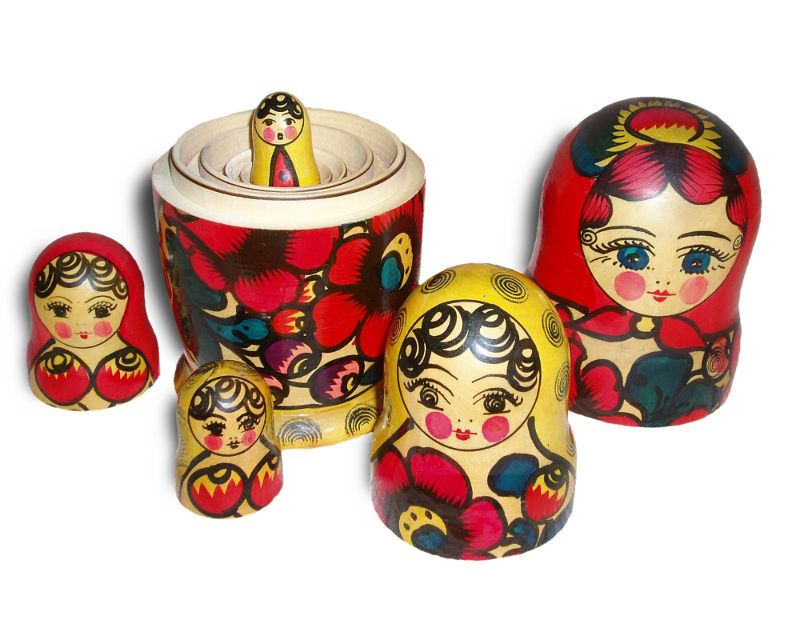
\includegraphics[width=0.8\textwidth]{images/matroska.jpg}
  \end{center}
\end{frame}

\begin{frame}
  \frametitle{Какво е рекурсия?}

  \begin{center}
    
\includegraphics[width=0.9\textwidth]{images/sierpinski.png}
  \end{center}
\end{frame}

\begin{frame}
  \frametitle{Какво е рекурсия?}

  \pause
  Повторение чрез позоваване на себе си
  \vspace{1em}

  \pause
  Рекурсивна функция: дефинира се чрез себе си

  \begin{equation*}
    n! = \left\{
    \begin{array}{l@{}l@{\qquad}l}
      1,&\text{ при }n = 0,&\textbf{(база)}\\
      n\cdot (n-1)!,&\text{ при }n > 0.&\textbf{(стъпка)}
    \end{array}\right.
  \end{equation*}
  \vspace{1em}

  \pause

  \begin{itemize}
  \item Дава се отговор на най-простата задача (база, дъно)
  \item Показва се как сложна задача се свежда към една или няколко по-прости задачи от същия вид (стъпка)
  \end{itemize}
\end{frame}


\begin{frame}
  \frametitle{Рекурсивни уравнения}

  Какво означава ``да дефинираме функция чрез себе си''?
  \vspace{1em}

  \pause

  Да разгледаме \emph{рекурсивното уравнение}, в което $F$ е неизвестно:
  \begin{equation*}
    F(n) =
    \underbrace{\begin{cases}
      1,&\text{ при }n = 0,\\
      n \cdot F(n-1),&\text{ при }n > 0.
    \end{cases}}_{\Gamma(F)(n)}
  \end{equation*}

  \pause
  \alert{$n!$ е ``най-малкото'' решение на уравнението $F = \Gamma(F)$.}
\end{frame}

\begin{frame}[fragile]
  \frametitle{Най-малка неподвижна точка}

  \begin{theorem}[Knaster-Tarski]
    Ако $\Gamma$ е изчислим оператор, то уравнението $F = \Gamma(F)$ има единствено най-малко решение $f$ \pause (\textbf{най-малка неподвижна точка на $\Gamma$}). \pause Нещо повече, решението точно съответства на рекурсивна програма пресмятаща $f$ чрез $\Gamma$.
  \end{theorem}

  \pause

\begin{verbatim}
(define (fact n)
  (if (= n 0) 1
      (* n (fact (- n 1)))))
\end{verbatim}

  \pause

  Кое е \textbf{най-малкото решение} на уравнението $F(x) = 1 + F(x-1)$?

  \pause

\verb#(define (f x) (+ 1 (f (- x 1)))#\\
\evalsto{(f 0)}?

  \pause

  $f$ е ``празната функция'', т.е. $\mathrm{dom}(f) = \emptyset$.

\end{frame}

\begin{frame}
  \frametitle{Операционна и денотационна семантика}

  Два подхода за описание на смисъла на функциите в Scheme.
  \pause

  Нека \tt{(define (f x) $\Gamma$[f])} е рекурсивно дефинирана функция.
  \pause

  \alert{Коя е математическата функция $f$, която се пресмята от \tt f?}
  \vspace{1em}

  \pause
  \textbf{Денотационна семантика}

  $f$ е най-малката неподвижна точка на уравнението $F = \Gamma(F)$.

  \vspace{1em}

  \pause
  \textbf{Операционна семантика}

  Разглеждаме редицата от последователни оценки на комбинацията\\
  \tt{(f a)} $\rightarrow$ \tt{$\Gamma$[f][x $\mapsto$ a]} $\rightarrow\ldots$.\\
  Ако редицата завършва с атома \tt b, дефинираме $f(a) := b$.
  \pause
  \vspace{1em}

  \alert{Функциите в Scheme имат дуален, но еквивалентен смисъл:}
  \begin{itemize}
  \item решения на рекурсивни уравнения
  \item изчислителни процеси, генериращи се при оценка
  \end{itemize}
\end{frame}


\subsection{Рекурсивни процеси}

\begin{frame}
  \frametitle{Оценка на рекурсивна функция}

  \begin{center}
    \footnotesize
    \begin{tabular}{c}
      \tt{(fact 4)}\\
      \pause
      \nxt{\bda\\
      \alt<+->{\tt{(* 4 (fact 3))}}{\tt{(if (= 4 0) 1 (* 4 (fact (- 4 1))))}}\\
      \nxt{\bda\\
      \alt<+->{\tt{(* 4 (* 3 (fact 2)))}}{\tt{(* 4 (if (= 3 0) 1 (* 3 (fact (- 3 1)))))}}\\
      \nxt{\bda\\
      \alt<+->{\tt{(* 4 (* 3 (* 2 (fact 1))))}}{\tt{(* 4 (* 3 (if (= 2 0) 1 (* 2 (fact (- 2 1))))))}}\\
      \nxt{\bda\\
      \alt<+->{\tt{(* 4 (* 3 (* 2 (* 1 (fact 0)))))}}{\tt{(* 4 (* 3 (* 2 (if (= 1 0) 1 (* 1 (fact (- 1 1)))))))}}\\
      \nxt{\bda\\
      \tt{(* 4 (* 3 (* 2 (* 1 1))))}\\
      \nxt{\bda\\
      \tt{(* 4 (* 3 (* 2 1)))}\\
      \nxt{\bda\\
      \tt{(* 4 (* 3 2))}\\
      \nxt{\bda\\
      \tt{(* 4 6)}\\
      \nxt{\bda\\
      24}}}}}}}}}
    \end{tabular}
  \end{center}
\end{frame}

\begin{frame}
  \frametitle{Оценка на рекурсивна функция в среда}

  {
  \tiny
  \begin{columns}[t,onlytextwidth]
    \column{0.63\textwidth}
    {}

    \begin{tabular}{lc}
      \nxt{
      \inenv E&\tt{(fact 4)}\\
      \nxt{&\bda\\
      \inenv{E_1}&\alt<+->{\tt{(* 4 (fact 3))}}{\tt{(if (= n 0) 1 (* n (fact (- n 1))))}}\\
      \nxt{&\bda\\
      \inenv{E_2}&\alt<+->{\tt{(* 4 (* 3 (fact 2)))}}{\tt{(* 4 (if (= n 0) 1 (* n (fact (- n 1)))))}}\\
      \nxt{&\bda\\
      \inenv{E_3}&\alt<+->{\tt{(* 4 (* 3 (* 2 (fact 1))))}}{\tt{(* 4 (* 3 (if (= n 0) 1 (* n (fact (- n 1))))))}}\\
      \nxt{&\bda\\
      \inenv{E_4}&\alt<+->{\tt{(* 4 (* 3 (* 2 (* 1 (fact 0)))))}}{\tt{(* 4 (* 3 (* 2 (if (= n 0) 1 (* n (fact (- n 1)))))))}}\\
      \nxt{&\bda\\
      \alt<+->{\inenv{E_4}&\tt{(* 4 (* 3 (* 2 (* 1 1))))}}{\inenv{E_5}&\tt{(* 4 (* 3 (* 2 (* 1 (if (= n 0) 1 (* n (fact (- n 1))))))))}}\\
      \nxt{&\bda\\
      \inenv{E_3}&\tt{(* 4 (* 3 (* 2 1)))}\\
      \nxt{&\bda\\
      \inenv{E_2}&\tt{(* 4 (* 3 2))}\\
      \nxt{&\bda\\
      \inenv{E_1}&\tt{(* 4 6)}\\
      \nxt{&\bda\\
      \inenv E&24}}}}}}}}}}
    \end{tabular}

    \column{0.37\textwidth}
    {}

    \begin{tabular}{*{8}{c@{}}c}
      \multicolumn{9}c{
      \begin{envir}{E}
        \\\firstinenv &&\\[1pt]\hspace{6ex}\tt{fact}&:&\funcenv n\ldots E
      \end{envir}}
      \\
      \multicolumn 2c{\visible<2->{\Bigg\uparrow}}&
      \visible<8->{\Bigg\uparrow}&
      \multicolumn 3c{\visible<4->{\Bigg\uparrow}}&
      \visible<10->{\Bigg\uparrow}&
      \multicolumn 2c{\visible<6->{\Bigg\uparrow}}\\
      \multicolumn 2c{
      \visible<2->{
      \begin{envir}{E_1}
        \\\firstinenv\tt n&:&4
      \end{envir}}}&
      \visible<8->{\Bigg\vert}&
      \multicolumn 3c{
      \visible<4->{
      \begin{envir}{E_2}
        \\\firstinenv\tt n&:&3
      \end{envir}}}&
      \visible<10->{\Bigg\vert}&
      \multicolumn 2c{
      \visible<6->{
      \begin{envir}{E_3}
        \\\firstinenv\tt n&:&2
      \end{envir}}}\\
      \multicolumn 2c{}&
      \visible<8->{\Bigg\vert}&
      \multicolumn 3c{}&
      \visible<10->{\Bigg\vert}&
      \multicolumn 2c{}\\
      &
      \multicolumn 3c{
      \visible<8->{
      \hspace{5ex}
      \begin{envir}{E_4}
        \\\firstinenv\tt n&:&1
      \end{envir}}}&&
      \multicolumn 3c{
      \visible<10->{
      \hspace{2ex}
      \begin{envir}{E_5}
        \\\firstinenv\tt n&:&0
      \end{envir}}}&
    \end{tabular}
  \end{columns}
  }
  \vspace{1em}

  \nxt{Линеен рекурсивен процес}
\end{frame}

\subsection{Итеративни процеси}


\begin{frame}[fragile]
  \frametitle{Факториел с цикъл}

  \begin{columns}[t,onlytextwidth]
    \column{0.5\textwidth}
    Факториел на C++

\begin{semiverbatim}
\only<3>\fbox{int fact(int n)} \{
  \only<4>\fbox{int r = 1;}
  for(\only<5>\fbox{int i = 1}; \only<6>\fbox{i <= n}; \only<7>\fbox{i++})
    \only<8>\fbox{r *= i;}
  \only<9>\fbox{return r;}
\}
\end{semiverbatim}

  \pause

    \column{0.5\textwidth}
    Превод на Scheme

\begin{semiverbatim}
(define (for n \only<4,8>\fbox{r} \only<5,7>\fbox{i})
  (if \only<6>\fbox{(<= i n)}
      (for n \only<8>\fbox{(* r i)} \only<7>\fbox{(+ i 1)})
      \only<9>\fbox{r}))

\only<3>\fbox{(define (fact n)}
  (for n \only<4>\fbox{1} \only<5>\fbox{1}))
\end{semiverbatim}
  \end{columns}
\end{frame}

\begin{frame}
  \frametitle{Оценка на итеративен факториел}

  \begin{center}
    \small
    \begin{tabular}{c}
      \nxt{\tt{(fact 4)}\\
      \nxt{\bda\\
      \tt{(for 4 1 1)}\\
      \nxt{\bda\\
      \alt<+->{\tt{(for 4 1 2)}}{\tt{(if (<= 1 4) (for 4 (* 1 1) (+ 1 1)) 1)}}\\
      \nxt{\bda\\
      \alt<+->{\tt{(for 4 2 3)}}{\tt{(if (<= 2 4) (for 4 (* 1 2) (+ 2 1)) 2)}}\\
      \nxt{\bda\\
      \alt<+->{\tt{(for 4 6 4)}}{\tt{(if (<= 3 4) (for 4 (* 2 3) (+ 3 1)) 6)}}\\
      \nxt{\bda\\
      \alt<+->{\tt{(for 4 24 5)}}{\tt{(if (<= 4 4) (for 4 (* 6 4) (+ 4 1)) 24)}}\\
      \nxt{\bda\\
      \alt<+->{\tt{24}}{\tt{(if (<= 5 4) (for 4 (* 24 5) (+ 5 1)) 24)}}}}}}}}}
    \end{tabular}
  \end{center}
  \vspace{1em}

  \nxt{Линеен итеративен процес}
\end{frame}

\begin{frame}<1-13>[label=iterenv]
  \frametitle{Оценка на итеративен факториел със среди}

  \begin{columns}[t,onlytextwidth]
    \column{0.6\textwidth}
    {}

    \scriptsize
    \begin{tabular}{lc}
      \nxt{\inenv E&\tt{(fact 4)}\\
      &\nxt{\bda\\
      \inenv{E_0}&\alt<+->{\tt{(for \alert<14>4 1 1)}}{\tt{(for n 1 1)}}\\
      &\nxt{\bda\\
      \inenv{E_1}&\alt<+->{\tt{(for \alert<14>4 1 2)}}{\tt{(if (<= i n) (for n (* r i) (+ i 1)) r)}}\\
      &\nxt{\bda\\
      \inenv{E_2}&\alt<+->{\tt{(for \alert<14>4 2 3)}}{\tt{(if (<= i n) (for n (* r i) (+ i 1)) r)}}\\
      &\nxt{\bda\\
      \inenv{E_3}&\alt<+->{\tt{(for \alert<14>4 6 4)}}{\tt{(if (<= i n) (for n (* r i) (+ i 1)) r)}}\\
      &\nxt{\bda\\
      \inenv{E_4}&\alt<+->{\tt{(for \alert<14>4 24 5)}}{\tt{(if (<= i n) (for n (* r i) (+ i 1)) r)}}\\
      &\nxt{\bda\\
      \inenv{E_5}&\alt<+->{\tt{24}}{\tt{(if (<= i n) (for n (* r i) (+ i 1)) r)}}}}}}}}}
    \end{tabular}

    \column{0.4\textwidth}
    {}

    \tiny
    \begin{tabular}{*{8}{c@{}}c}
      \multicolumn 9c{
      \visible<2->{
      \begin{envir}{E_0}
        \\\firstinenv \tt n&:&4
      \end{envir}}}
      \\
      \multicolumn 9c{\visible<2->{\big\downarrow}}\\
      \multicolumn 9c{
      \begin{envir}{E}
        \\\firstinenv &&\\[1pt]\tt{fact}&:&\funcenv n{(for n 1 1)}E\\
        \tt{for}&:&\funcenv{\alert<14>n r i}\ldots E
      \end{envir}}
      \\
      \multicolumn 2c{\visible<4->\bua}&
      \visible<10->\bua&
      \multicolumn 3c{\visible<6->\bua}&
      \visible<12->\bua&
      \multicolumn 2c{\visible<8->\bua}\\
      \multicolumn 2c{
      \visible<4->{
      \begin{envir}{E_1}
        \\\firstinenv\alert<14>{\tt n}&\alert<14>:&\alert<14>4\\
        \tt r&:&1\\
        \tt i&:&1
      \end{envir}}}&
      \visible<10->{
      \begin{tabular}{@{}c@{}}
      \!\!\Bigg\vert\\[0pt]
      \!\!\bigg\vert
      \end{tabular}}&
      \multicolumn 3c{
      \visible<6->{
      \begin{envir}{E_2}
        \\\firstinenv\alert<14>{\tt n}&\alert<14>:&\alert<14>4\\
        \tt r&:&1\\
        \tt i&:&2
      \end{envir}}}&
      \visible<12->{
      \begin{tabular}{@{}c@{}}
      \!\!\Bigg\vert\\[0pt]
      \!\!\bigg\vert
      \end{tabular}}&
      \multicolumn 2c{
      \visible<8->{
      \begin{envir}{E_3}
        \\\firstinenv\alert<14>{\tt n}&\alert<14>:&\alert<14>4\\
        \tt r&:&2\\
        \tt i&:&3
      \end{envir}}}\\
      \multicolumn 2c{}&
      \visible<10->{\big\vert}&
      \multicolumn 3c{}&
      \visible<12->{\big\vert}&
      \multicolumn 2c{}\\
      &
      \multicolumn 3c{
      \visible<10->{
      \hspace{5ex}
      \begin{envir}{E_4}
        \\\firstinenv\alert<14>{\tt n}&\alert<14>:&\alert<14>4\\
        \tt r&:&6\\
        \tt i&:&4
      \end{envir}}}&&
      \multicolumn 3c{
      \visible<12->{
      \hspace{2ex}
      \begin{envir}{E_5}
        \\\firstinenv\alert<14>{\tt n}&\alert<14>:&\alert<14>4\\
        \tt r&:&24\\
        \tt i&:&5
      \end{envir}}}&
    \end{tabular}

  \end{columns}
\end{frame}

\begin{frame}<1-2>[fragile,label=reciter]
  \frametitle{Рекурсивен и итеративен процес}

  \begin{columns}[t,onlytextwidth]

    \column{0.5\textwidth}
    {}

    \begin{center}

      \tiny
      \begin{tabular}{c}
        \tt{(fact 4)} \\
        \bda\\
        \tt{(* 4 (fact 3))}\\
        \bda\\
        \tt{(* 4 (* 3 (fact 2)))}\\
        \bda\\
        \tt{(* 4 (* 3 (* 2 (fact 1))))}\\
        \bda\\
        \tt{(* 4 (* 3 (* 2 (* 1 (fact 0)))))}\\
        \bda\\
        \tt{(* 4 (* 3 (* 2 (* 1 1))))}\\
        \bda\\
        \tt{(* 4 (* 3 (* 2 1)))}\\
        \bda\\
        \tt{(* 4 (* 3 2))}\\
        \bda\\
        \tt{(* 4 6)}\\
        \bda\\
        24
      \end{tabular}
    \end{center}

    \scriptsize
    
\begin{semiverbatim}
    (define (fact n)
      (if (= n 0) 1
          \alert<2>{(* n }(fact (- n 1)))))
\end{semiverbatim}

    \column{0.5\textwidth}
    {}

    \begin{center}
      \tiny
      \begin{tabular}{c}
        \tt{(fact 4)}\\
        \bda\\
        \tt{(for \alert<3> 4 1 1)}\\
        \bda\\
        \tt{(for \alert<3> 4 1 2)}\\
        \bda\\
        \tt{(for \alert<3> 4 2 3)}\\
        \bda\\
        \tt{(for \alert<3> 4 6 4)}\\
        \bda\\
        \tt{(for \alert<3> 4 24 5)}\\
        \bda\\
        \tt{24}
      \end{tabular}
    \end{center}

    \scriptsize

\begin{semiverbatim}
(define (for \alert<3>n r i)
  (if (<= i n)
      (for \alert<3>n (* r i) (+ i 1))
      r))

(define (fact n)
  (for \alert<3>n 1 1))
\end{semiverbatim}

  \end{columns}
\end{frame}

\begin{frame}
  \frametitle{Опашкова рекурсия}

  \begin{itemize}[<+->]
  \item Функциите, в които има отложени операции генерират същински \textbf{рекурсивни процеси}
  \item Рекурсивно извикване, при което няма отложена операция се нарича \textbf{опашкова рекурсия}
  \item Функциите, в които всички рекурсивни извиквания са опашкови генерират \textbf{итеративни процеси}
  \item При итеративните процеси липсва етап на свиването на рекурсията
  \item Опашковата рекурсия се използва за симулиране на цикли
  \item В Scheme опашковата рекурсия \alert{по стандарт} се интерпретира като цикъл
    \begin{itemize}
    \item т.е. не се заделя памет за всяко рекурсивно извикване
    \end{itemize}
  \end{itemize}
\end{frame}

\section{Вложени дефиниции}

\againframe<3>{reciter}

\againframe<14>{iterenv}

\subsection{Влагане на \tt{define}}

\begin{frame}[fragile]
  \frametitle{Вложени дефиниции}

  \begin{itemize}
  \item \tta{(define (}<функция> \{<параметър\}\tta) \{<дефиниция>\} <тяло>\tta)
  \item При извикване на <функция> първо се оценяват всички <дефиниция> и след това се оценява <тяло>
  \item Вложените дефиниции се оценяват и записват в средата, която се \textbf{оценява} функцията, а не в средата, в която е \textbf{дефинирана}
  \item Пример:\\
\begin{verbatim}
(define (dist x1 y1 x2 y2)
  (define dx (- x2 x1))
  (define dy (- y2 y1))
  (define (sq x) (* x x))
  (sqrt (+ (sq dx) (sq dy))))
\end{verbatim}
  \end{itemize}
\end{frame}

\begin{frame}
  \frametitle{Оценка на вложени функции}

  \scriptsize
  \begin{columns}[t,onlytextwidth]
    \column{0.5\textwidth}
    {}

    \begin{tabular}{rc}
      \nxt{\inenv E&\tt{(dist 2 5 -1 9)}\\
      &\nxt{\nxt{\bda\\
      \inenv{E_1}&\tt{(define dx (- x2 x1))}\\
      \nxt{\inenv{E_1}&\tt{(define dy (- y2 y1))}\\
      \nxt{\inenv{E_1}&\tt{(define sq (* x x))}\\
      \nxt{\inenv{E_1}&\tt{(sqrt (+ (sq dx) (sq dy)))}\\
      &\nxt{\bda\\
      \inenv{E_2}&\tt{(sqrt (+ (* x x) (sq dy)))}\\
      &\nxt{\bda\\
      \inenv{E_3}&\tt{(sqrt (+ 9 (* x x)))}\\
      &\nxt{\bda\\
      \inenv{E_1}&\tt{(sqrt (+ 9 16))}\\
      &\nxt{\bda\\
      \inenv{E_1}&\tt{(sqrt 25)}\\
      &\nxt{\bda\\
      \inenv{E_1}&\tt 5}}}}}}}}}}}
    \end{tabular}

    \column{0.5\textwidth}
    {}

    \begin{tabular}{cc}
      \multicolumn 2c{
      \begin{envir}E
        \\\firstinenv \tt{dist}&:&\funcenv{x1 y1 x2 y2}\ldots E
      \end{envir}}
      \\
      \multicolumn 2c{\visible<2->\bua}
      \\
      \multicolumn 2c{\visible<2->{
      \begin{envir}{E_1}
        \\\firstinenv \tt{x1}&:&2
        \\\tt{y1}&:&5
        \\\tt{x2}&:&-1
        \\\tt{y2}&:&9
        \only<3->{\\\tt{dx}&:&3}
        \only<4->{\\\tt{dy}&:&4}
        \only<5->{\\\tt{sq}&:&\funcenv x{(* x x)}{E_1}}
      \end{envir}}}
      \\
      \only<7->\bua&\visible<8->\bua\\
      \only<7->{
      \begin{envir}{E_2}
        \\\firstinenv \tt x&:&3
      \end{envir}}&
      \only<8->{
      \begin{envir}{E_3}
        \\\firstinenv \tt x&:&4
      \end{envir}}
    \end{tabular}
  \end{columns}
\end{frame}

\begin{frame}[fragile]
  \frametitle{Вложена помощна итеративна функция}

  При итеративни функция е удобно помощната функция да е вложена.

\begin{semiverbatim}
\only<1>{(define (for n r i)
  (if (<= i n)
      (for n (* r i) (+ i 1))
      r))
}
(define (fact n)
\only<2->{  (define (for r i)
    (if (<= i n)
        (for (* r i) (+ i 1))
        r))
}  (for \only<1>{n }1 1))
\end{semiverbatim}

\onslide<3->{
  Вложените дефиниции ``виждат'' символите на обхващащите им дефиниции.
}
\end{frame}

\begin{frame}
  \frametitle{Оценка на итеративен факториел с вложена функция}

  \begin{columns}[t,onlytextwidth]
    \column{0.6\textwidth}
    {}

    \scriptsize
    \begin{tabular}{lc}
      \nxt{\inenv E&\tt{(fact 4)}\\
      &\nxt{\bda\\
      \inenv{E_0}&\alt<+->{\tt{(for 1 1)}}{\tt{(define (for r i) \ldots)}}\\
      &\nxt{\bda\\
      \inenv{E_1}&\alt<+->{\tt{(for 1 2)}}{\tt{(if (<= i n) (for (* r i) (+ i 1)) r)}}\\
      &\nxt{\bda\\
      \inenv{E_2}&\alt<+->{\tt{(for 2 3)}}{\tt{(if (<= i n) (for (* r i) (+ i 1)) r)}}\\
      &\nxt{\bda\\
      \inenv{E_3}&\alt<+->{\tt{(for 6 4)}}{\tt{(if (<= i n) (for (* r i) (+ i 1)) r)}}\\
      &\nxt{\bda\\
      \inenv{E_4}&\alt<+->{\tt{(for 24 5)}}{\tt{(if (<= i n) (for (* r i) (+ i 1)) r)}}\\
      &\nxt{\bda\\
      \inenv{E_5}&\alt<+->{\tt{24}}{\tt{(if (<= i n) (for (* r i) (+ i 1)) r)}}}}}}}}}
    \end{tabular}

    \column{0.4\textwidth}
    {}

    \tiny
    \begin{tabular}{*{8}{c@{}}c}
      \multicolumn 9c{
      \begin{envir}{E}
        \\\firstinenv &&\\[1pt]\tt{fact}&:&\funcenv n{(for 1 1)}E
      \end{envir}}
      \\
      \multicolumn 9c{\visible<2->\bua}
      \\
      \multicolumn 9c{
      \visible<2->{
      \begin{envir}{E_0}
        \\\firstinenv \tt n&:&4\\
        \hspace{6ex}\tt{for}&:&\funcenv{r i}\ldots {\alert<2>{E_0}}
      \end{envir}}}
      \\
      \multicolumn 2c{\visible<4->\bua}&
      \visible<10->\bua&
      \multicolumn 3c{\visible<6->\bua}&
      \visible<12->\bua&
      \multicolumn 2c{\visible<8->\bua}\\
      \multicolumn 2c{
      \visible<4->{
      \begin{envir}{E_1}
        \\\firstinenv\tt r&:&1\\
        \tt i&:&1
      \end{envir}}}&
      \visible<10->{
      \begin{tabular}{@{}c@{}}
      \!\!\Bigg\vert\\[0pt]
      \!\!\big\vert
      \end{tabular}}&
      \multicolumn 3c{
      \visible<6->{
      \begin{envir}{E_2}
        \\\firstinenv\tt r&:&1\\
        \tt i&:&2
      \end{envir}}}&
      \visible<12->{
      \begin{tabular}{@{}c@{}}
      \!\!\Bigg\vert\\[0pt]
      \!\!\big\vert
      \end{tabular}}&
      \multicolumn 2c{
      \visible<8->{
      \begin{envir}{E_3}
        \\\firstinenv\tt r&:&2\\
        \tt i&:&3
      \end{envir}}}\\
      \multicolumn 2c{}&
      \visible<10->{\big\vert}&
      \multicolumn 3c{}&
      \visible<12->{\big\vert}&
      \multicolumn 2c{}\\
      &
      \multicolumn 3c{
      \visible<10->{
      \hspace{5ex}
      \begin{envir}{E_4}
        \\\firstinenv\tt r&:&6\\
        \tt i&:&4
      \end{envir}}}&&
      \multicolumn 3c{
      \visible<12->{
      \hspace{2ex}
      \begin{envir}{E_5}
        \\\firstinenv\tt r&:&24\\
        \tt i&:&5
      \end{envir}}}&
    \end{tabular}
  \end{columns}
\end{frame}

\subsection{\tt{let} и \tt{let*}}

\begin{frame}
  \frametitle{Специална форма \tt{let}}

  \begin{itemize}[<+->]
  \item \tta{(let} \tta(\{\tta({}<символ> <израз>\tta)\}\tta) <тяло>\tt)
  \item \tta{(let ((}{}<символ$_1$> <израз$_1$>\tta)\\
    \tta{\hskip 7ex(}{}<символ$_2$> <израз$_2$>\tta)\\
    \hskip 7ex\ldots\\
    \tta{\hskip 7ex(}{}<символ$_n$> <израз$_n$>\tta{))}\\
    \hskip 7ex{}<тяло>\tta)
  \item При оценка на \tt{let} в среда \env E:
    \begin{itemize}[<+->]
    \item Създава се нова среда \env{E_1} разширение на текущата
      среда \env E
    \item Оценката на <израз$_1$> в \env E се свързва със <символ$_1$> в \env{E_1}
    \item Оценката на <израз$_2$> в \env E се свързва със <символ$_2$> в \env{E_1}
    \item \ldots
    \item Оценката на <израз$_n$> в \env E се свързва със <символ$_n$> в \env{E_1}
    \item Връща се оценката на <тяло> в средата \env{E_1}
    \end{itemize}
  \item \alert{\tt{let} няма странични ефекти върху средата!}
    \begin{itemize}
    \item за разлика от \tt{define}
    \end{itemize}
  \end{itemize}
\end{frame}

\begin{frame}<1-3>[fragile]
  \frametitle{Пример за \tt{let}}

\begin{verbatim}
(define (dist x1 y1 x2 y2)
  (let ((dx (- x2 x1))
        (dy (- y2 y1)))
   (sqrt (+ (sq dx) (sq dy)))))
\end{verbatim}

\pause
\begin{semiverbatim}
(define (area x1 y1 x2 y2 x3 y3)
  (let ((a (dist x1 y1 x2 y2))
        (b (dist x2 y2 x3 y3))
        (c (dist x3 y3 x1 y1))
        \alert<3>{(p (/ (+ a b c) 2))})
   (sqrt (* p (- p a) (- p b) (- p c)))))
\end{semiverbatim}
\end{frame}

\begin{frame}
  \frametitle{Оценка на \tt{let}}

  \scriptsize
  \begin{columns}[t,onlytextwidth]
    \column{0.5\textwidth}
    {}

    \begin{tabular}{rc}
      \nxt{\inenv E&\tt{(dist 2 5 -1 9)}\\
      &\nxt{\bda\\
      \inenv{E_1}&\begin{tabular}{l}
                    \tt{(let ((dx (- x2 x1))}\\
                    \tt{\hskip 7ex(dy (- y2 y1)))}\\
                    \tt{ (sqrt (+ (sq dx) (sq dy))))}
                  \end{tabular}\\
      &\nxt{\bda\\
      \inenv{E_2}&\tt{(sqrt (+ (sq dx) (sq dy)))}\\
      &\nxt{\bda\\
      \inenv{E_3}&\tt{(sqrt (+ (* x x) (sq dy)))}\\
      &\nxt{\bda\\
      \inenv{E_4}&\tt{(sqrt (+ 9 (* x x)))}\\
      &\nxt{\bda\\
      \inenv{E_2}&\tt{(sqrt (+ 9 16))}\\
      &\nxt{\bda\\
      \inenv{E_2}&\tt{(sqrt 25)}\\
      &\nxt{\bda\\
      \inenv{E_2}&\tt 5}}}}}}}}
    \end{tabular}

    \column{0.5\textwidth}
    {}

    \begin{tabular}{ccc}
      \multicolumn 3c{
      \begin{envir}E
        \\\firstinenv \tt{dist}&:&\funcenv{x1 y1 x2 y2}\ldots E
      \end{envir}}
      \\
      \onslide<7->\bua&\only<2->\bua&\onslide<8->\bua\\
      \onslide<7->{
      \begin{envir}{E_3}
        \\\firstinenv \tt x&:&3
      \end{envir}}&
      \onslide<2->{
      \begin{envir}{E_1}
        \\\firstinenv \tt{x1}&:&2
        \\\tt{y1}&:&5
        \\\tt{x2}&:&-1
        \\\tt{y2}&:&9
      \end{envir}}&
      \onslide<8->{
      \begin{envir}{E_4}
        \\\firstinenv \tt x&:&4
      \end{envir}}\\
      \multicolumn 3c{\visible<3->\bua}\\
      \multicolumn 3c{\visible<3->{
      \begin{envir}{E_2}
        \\\firstinenv \tt{dx}&:&3
        \\\tt{dy}&:&4
      \end{envir}}}
    \end{tabular}
  \end{columns}
\end{frame}

\begin{frame}
  \frametitle{Специална форма \tt{let*}}

  \begin{itemize}[<+->]
  \item \tta{(let*} \tta(\{\tta({}<символ> <израз>\tta)\}\tta) <тяло>\tt)
  \item \tta{(let* ((}{}<символ$_1$> <израз$_1$>\tta)\\
    \tta{\hskip 8ex(}{}<символ$_2$> <израз$_2$>\tta)\\
    \hskip 7ex\ldots\\
    \tta{\hskip 8ex(}{}<символ$_n$> <израз$_n$>\tta{))}\\
    \tta{\hskip 8ex}{}<тяло>\tta)
  \item При оценка на \tt{let*} в среда \env E:
    \begin{itemize}[<+->]
    \item Създава се нова среда \env{E_1} разширение на текущата
      среда \env E
    \item Оценката на <израз$_1$> в \env E се свързва със <символ$_1$> в \env{E_1}
    \item Създава се нова среда \env{E_2} разширение на текущата
      среда \env{E_1}
    \item Оценката на <израз$_2$> в \env{E_1} се свързва със <символ$_2$> в \env{E_2}
    \item \ldots
    \item Създава се нова среда \env{E_n} разширение на текущата
      среда \env{E_{n-1}}
    \item Оценката на <израз$_n$> в \env{E_{n-1}} се свързва със <символ$_n$> в \env{E_n}
    \item Връща се оценката на <тяло> в средата \env{E_n}
    \end{itemize}
  \end{itemize}
\end{frame}

\begin{frame}[fragile]
  \frametitle{Пример за \tt{let*}}

\begin{verbatim}
(define (area x1 y1 x2 y2 x3 y3)
  (let* ((a (dist x1 y1 x2 y2))
         (b (dist x2 y2 x3 y3))
         (c (dist x3 y3 x1 y1))
         (p (/ (+ a b c) 2)))
   (sqrt (* p (- p a) (- p b) (- p c)))))
\end{verbatim}

\pause

\begin{semiverbatim}
(define (area x1 y1 x2 y2 x3 y3)
  (let* (\alert{(p (/ (+ a b c) 2))}
         (a (dist x1 y1 x2 y2))
         (b (dist x2 y2 x3 y3))
         (c (dist x3 y3 x1 y1)))
   (sqrt (* p (- p a) (- p b) (- p c)))))
\end{semiverbatim}
\end{frame}

\begin{frame}
  \frametitle{Оценка на \tt{let*}}

  \scriptsize
  \begin{columns}[t,onlytextwidth]
    \column{0.5\textwidth}
    {}

    \begin{tabular}{rc}
      \nxt{\inenv E&\tt{(dist 2 5 -1 9)}\\
      &\nxt{\bda\\
      \inenv{E_1}&\begin{tabular}{l}
                    \tt{(let ((dx (- x2 x1))}\\
                    \tt{\hskip 7ex(dy (- y2 y1)))}\\
                    \tt{ (sqrt (+ (sq dx) (sq dy))))}
                  \end{tabular}\\
      &\nxt{\nxt{\bda\\
      \inenv{E_3}&\tt{(sqrt (+ (sq dx) (sq dy)))}\\
      &\nxt{\bda\\
      \inenv{E_4}&\tt{(sqrt (+ (* x x) (sq dy)))}\\
      &\nxt{\bda\\
      \inenv{E_5}&\tt{(sqrt (+ 9 (* x x)))}\\
      &\nxt{\bda\\
      \inenv{E_3}&\tt{(sqrt (+ 9 16))}\\
      &\nxt{\bda\\
      \inenv{E_3}&\tt{(sqrt 25)}\\
      &\nxt{\bda\\
      \inenv{E_3}&\tt 5}}}}}}}}}
    \end{tabular}

    \column{0.5\textwidth}
    {}

    \begin{tabular}{ccc}
      \multicolumn 3c{
      \begin{envir}E
        \\\firstinenv \tt{dist}&:&\funcenv{x1 y1 x2 y2}\ldots E
      \end{envir}}
      \\
      \onslide<7->\bua&\only<2->\bua&\onslide<8->\bua\\
      \onslide<7->{
      \begin{envir}{E_4}
        \\\firstinenv \tt x&:&3
      \end{envir}}&
      \onslide<2->{
      \begin{envir}{E_1}
        \\\firstinenv \tt{x1}&:&2
        \\\tt{y1}&:&5
        \\\tt{x2}&:&-1
        \\\tt{y2}&:&9
      \end{envir}}&
      \onslide<8->{
      \begin{envir}{E_5}
        \\\firstinenv \tt x&:&4
      \end{envir}}\\
      \multicolumn 3c{\visible<3->\bua}\\
      \multicolumn 3c{\visible<3->{
      \begin{envir}{E_2}
        \\\firstinenv \tt{dx}&:&3
      \end{envir}}}\\
      \multicolumn 3c{\visible<4->\bua}\\
      \multicolumn 3c{\visible<4->{
      \begin{envir}{E_3}
        \\\firstinenv \tt{dy}&:&4
      \end{envir}}}
    \end{tabular}
  \end{columns}
\end{frame}

\section{Нелинейни изчислителни процеси}

\subsection{Логаритмични процеси}

\begin{frame}[fragile]
  \frametitle{Степенуване}

  Функцията $x^n$ може да се дефинира по следния начин:
  \begin{equation*}
    x^n = \begin{cases}
      1,&\text{ ако }n = 0,\\
      \frac 1 {x^{-n}},&\text{ ако }n < 0,\\
      x\cdot x^{n-1},&\text{ ако }n > 0.
    \end{cases}
  \end{equation*}

  \pause

\begin{verbatim}
(define (pow x n)
  (cond ((= n 0) 1)
        ((< n 0) (/ 1 (pow x (- n))))
        (else (* x (pow x (- n 1))))))
\end{verbatim}
\end{frame}

\begin{frame}
  \frametitle{Оценка на степенуване}

  \begin{center}
    \tiny
    \begin{tabular}{c}
      \tt{(pow 2 6)}\\
      \nxt{\bda\\
      \tt{(* 2 (pow 2 5))}\\
      \nxt{\bda\\
      \tt{(* 2 (* 2 (pow 2 4)))}\\
      \nxt{\bda\\
      \tt{(* 2 (* 2 (* 2 (pow 2 3))))}\\
      \nxt{\bda\\
      \tt{(* 2 (* 2 (* 2 (* 2 (pow 2 2)))))}\\
      \nxt{\bda\\
      \tt{(* 2 (* 2 (* 2 (* 2 (* 2 (pow 2 1))))))}\\
      \nxt{\bda\\
      \tt{(* 2 (* 2 (* 2 (* 2 (* 2 (* 2 (pow 2 0)))))))}\\
      \nxt{\bda\\
      \tt{(* 2 (* 2 (* 2 (* 2 (* 2 (* 2 1))))))}\\
      \nxt{\bda\\
      \tt{(* 2 (* 2 (* 2 (* 2 (* 2 2)))))}\\
      \nxt{\bda\\
      \tt{(* 2 (* 2 (* 2 (* 2 4))))}\\
      \nxt{\bda\\
      \tt{(* 2 (* 2 (* 2 8)))}\\
      \nxt{\bda\\
      \tt{(* 2 (* 2 16))}\\
      \nxt{\bda\\
      \tt{(* 2 32)}\\
      \nxt{\bda\\
      \tt{64}}}}}}}}}}}}}}
    \end{tabular}
  \end{center}

  \nxt{Линеен рекурсивен процес}
\end{frame}

\begin{frame}[fragile]
  \frametitle{Бързо степенуване}

  Алтернативна дефиниция на $x^n$:
  \begin{equation*}
    x^n = \begin{cases}
      1,&\text{ ако }n = 0,\\
      \frac 1 {x^{-n}},&\text{ ако }n < 0,\\
      (x^{\frac n2})^2,&\text{ ако }n > 0, n\text{ --- четно},\\
      x\cdot x^{n-1},&\text{ ако }n > 0, n\text{ --- нечетно}.
    \end{cases}
  \end{equation*}

  \pause

\begin{verbatim}
(define (qpow x n)
  (define (sqr x) (* x x))
  (cond ((= n 0) 1)
        ((< n 0) (/ 1 (qpow x (- n))))
        ((even? n) (sqr (qpow x (quotient n 2))))
        (else (* x (qpow x (- n 1))))))
\end{verbatim}
\end{frame}

\begin{frame}
  \frametitle{Оценка на бързо степенуване}

  \begin{center}
    \scriptsize
    \begin{tabular}{c}
      \tt{(qpow 2 6)}\\
      \nxt{\bda\\
      \tt{(sqr (qpow 2 3))}\\
      \nxt{\bda\\
      \tt{(sqr (* 2 (qpow 2 2)))}\\
      \nxt{\bda\\
      \tt{(sqr (* 2 (sqr (qpow 2 1))))}\\
      \nxt{\bda\\
      \tt{(sqr (* 2 (sqr (* 2 (qpow 2 0)))))}\\
      \nxt{\bda\\
      \tt{(sqr (* 2 (sqr (* 2 1))))}\\
      \nxt{\bda\\
      \tt{(sqr (* 2 (sqr 2)))}\\
      \nxt{\bda\\
      \tt{(sqr (* 2 4))}\\
      \nxt{\bda\\
      \tt{(sqr 8)}\\
      \nxt{\bda\\
      \tt{64}}}}}}}}}}
    \end{tabular}
  \end{center}

  \nxt{Логаритмичен рекурсивен процес}
\end{frame}

\subsection{Дървовидни рекурсивни процеси}

\begin{frame}[fragile]
  \frametitle{Числа на Фибоначи}

  $0, 1, 1, 2, 3, 5, 8, 13, 21, 34, 55, 89, 144, 233, 377, \ldots$

  \pause
  \begin{equation*}
    f_n =
    \begin{cases}
      0, &\text{ за }n = 0,\\
      1, &\text{ за }n = 1,\\
      f_{n-1} + f_{n-2}, &\text{ за }n \geq 2.
    \end{cases}
  \end{equation*}

  \pause

\begin{verbatim}
(define (fib n)
  (cond ((= n 0) 0)
        ((= n 1) 1)
        (else (+ (fib (- n 1)) (fib (- n 2))))))
\end{verbatim}

  \pause

  $f_{40} = ?$

\end{frame}

\begin{frame}
  \frametitle{Дървовидна рекурсия}

  \begin{center}
    \only<1>{
      \begin{forest} for tree={edge=->}
        [\tt{(fib 2)}
        [\tt{(fib 1)} [\tt 1]] [\tt{(fib 0)}
        [\tt 0]]]
      \end{forest}
    }
    \only<2>{
      \begin{forest} for tree={edge=->}
      [\tt{(fib 3)}
      [\tt{(fib 2)}
      [\tt{(fib 1)} [\tt 1]]
      [\tt{(fib 0)} [\tt 0]]]
      [\tt{(fib 1)} [\tt 1]]]
      \end{forest}
    }
    \only<3>{
      \begin{forest} for tree={edge=->}
      [\tt{(fib 4)}
      [\tt{(fib 3)}
      [\tt{(fib 2)}
      [\tt{(fib 1)} [\tt 1]]
      [\tt{(fib 0)} [\tt 0]]]
      [\tt{(fib 1)} [\tt 1]]]
      [\tt{(fib 2)}
      [\tt{(fib 1)} [\tt 1]]
      [\tt{(fib 0)} [\tt 0]]]]
      \end{forest}
    }
    \only<4>{
      \scriptsize
      \begin{forest} for tree={edge=->}
      [\tt{(fib 5)}
      [\tt{(fib 4)}
      [\tt{(fib 3)}
      [\tt{(fib 2)}
      [\tt{(fib 1)} [\tt 1]]
      [\tt{(fib 0)} [\tt 0]]]
      [\tt{(fib 1)} [\tt 1]]]
      [\tt{(fib 2)}
      [\tt{(fib 1)} [\tt 1]]
      [\tt{(fib 0)} [\tt 0]]]]
      [\tt{(fib 3)}
      [\tt{(fib 2)}
      [\tt{(fib 1)} [\tt 1]]
      [\tt{(fib 0)} [\tt 0]]]
      [\tt{(fib 1)} [\tt 1]]]]
      \end{forest}
    }
    \only<5->{
    \tiny
    \begin{forest} for tree={edge=->,s sep=1pt,inner sep=1pt}
      [\tt{(fib 6)}
      [\tt{(fib 5)}
      [\tt{(fib 4)}
      [\tt{(fib 3)}
      [\tt{(fib 2)}
      [\tt{(fib 1)} [\tt 1]]
      [\tt{(fib 0)} [\tt 0]]]
      [\tt{(fib 1)} [\tt 1]]]
      [\tt{(fib 2)}
      [\tt{(fib 1)} [\tt 1]]
      [\tt{(fib 0)} [\tt 0]]]]
      [\tt{(fib 3)}
      [\tt{(fib 2)}
      [\tt{(fib 1)} [\tt 1]]
      [\tt{(fib 0)} [\tt 0]]]
      [\tt{(fib 1)} [\tt 1]]]]
      [\tt{(fib 4)}
      [\tt{(fib 3)}
      [\tt{(fib 2)}
      [\tt{(fib 1)} [\tt 1]]
      [\tt{(fib 0)} [\tt 0]]]
      [\tt{(fib 1)} [\tt 1]]]
      [\tt{(fib 2)}
      [\tt{(fib 1)} [\tt 1]]
      [\tt{(fib 0)} [\tt 0]]]]]
    \end{forest}
    }
  \end{center}

  \onslide<6>{Дървовиден рекурсивен процес}
\end{frame}

\begin{frame}[fragile]
  \frametitle{Как да оптимизираме?}

  \textbf{Решение №1: мемоизация}

  Да помним вече пресметнатите стойности, вместо да ги смятаме пак.

  \pause
  \alert{За реализацията са нужни странични ефекти.}

  \pause
  \vspace{1em}

  \textbf{Решение №2: динамично програмиране}

  Строим последователно всички числа на Фибоначи в нарастващ ред.

  \pause
  \alert{Нужно е да помним само последните две числа!}

  \pause
\begin{verbatim}
(define (fib n)
  (define (iter i fib_i fib_i-1)
    (if (= i n) fib_i
        (iter (+ i 1) (+ fib_i fib_i-1) fib_i)))
  (if (= n 0) 0
      (iter 1 1 0)))
\end{verbatim}
\end{frame}

\begin{frame}
  \frametitle{Итеративно генериране на числата на Фибоначи}

  \small
  \begin{center}
    \begin{tabular}{c}
      \nxt{\tt{(fib 7)}\\
      \nxt{\bda\\
      \tt{(iter 1 1 0)}\\
      \nxt{\bda\\
      \tt{(iter 2 1 1)}\\
      \nxt{\bda\\
      \tt{(iter 3 2 1)}\\
      \nxt{\bda\\
      \tt{(iter 4 3 2)}\\
      \nxt{\bda\\
      \tt{(iter 5 5 3)}\\
      \nxt{\bda\\
      \tt{(iter 6 8 5)}\\
      \nxt{\bda\\
      \tt{(iter 7 13 8)}\\
      \nxt{\bda\\
      \tt{13}}}}}}}}}}
    \end{tabular}
  \end{center}
\end{frame}

\end{document}
